\documentclass{article}

%%%%%%%%%%%%%%%%%%%%%%%%%%%%%%%%%% Maths %%%%%%%%%%%%%%%%%%%%%%%%%%%%
\usepackage{amsmath}

%%%%%%%%%%%%%%%%%%%%%%%%%%%%%%%%%% referencing %%%%%%%%%%%%%%%%%%%%%%%%%%%%%%%%%%
\usepackage{natbib}
\usepackage{hyperref}
\usepackage{xcolor}
\hypersetup{
    colorlinks,
    %linkcolor={red!50!black},
    linkcolor={black},
    citecolor={blue!50!black},
    urlcolor={blue!80!black}
}

%%%%%%%%%%%%%%%%%%%%%%%%%%%%%%%%%% figure and table %%%%%%%%%%%%%%%%%%%%%%%%%%%%%%%%%%
\usepackage{graphicx}
\graphicspath{{./figures/}}
\usepackage{subfig}

%%%%%%%%%%%%%%%%%%%%%%%%%%%%%%%%%% layout %%%%%%%%%%%%%%%%%%%%%%%%%%%%%%%%%%
\usepackage{setspace}
\linespread{1.5}
\usepackage{fullpage}
\usepackage{authblk}

%\usepackage{fancyhdr}
\providecommand{\keywords}[1]{\textbf{\textit{Key words:}} #1}

%\newcommand\@shorttitle{}
% define \theshorttitle to what is given
%\newcommand\shorttitle[1]{\renewcommand\@shorttitle{#1}}

%%%%%%%%%%%%%%%%%%%%%%%%%%%%%%%%%% todo %%%%%%%%%%%%%%%%%%%%%%%%%%%%%%%%%%
%\usepackage[colorinlistoftodos]{todonotes}
\usepackage[disable]{todonotes}

\newcounter{todocounter}
\newcommand{\todonum}[2][]
{\stepcounter{todocounter}\todo[#1]{\thetodocounter: #2}}

\newcommand{\done}[2][]
{\todo[color=green!40, #1]{#2}}
\newcommand{\donenum}[2][]
{\stepcounter{todocounter}\done[#1]{\thetodocounter: #2}}


\newcommand{\narrative}[2][]
{\todo[color=blue!40, #1]{#2}}
\newcommand{\narrativenum}[2][]
{\stepcounter{todocounter}\narrative[#1]{\thetodocounter: #2}}


\begin{document}

\title{The rate and structure of mixed infections in global populations of {\it Plasmodium} malaria}
%\shorttitle{Global malaria mixed infection}
\newcommand\shorttitle{Global malaria mixed infection}
%\shorttitle
\date{}

\author{(LIST OF NAMES! NOT RIGHT ORDER)}
\author[1,2]{Sha Joe Zhu}
\author[1,2,3,4]{Jacob Almagro-Garcia}
\author[2]{Jason}
\author[1,3,4]{Richard}
\author[1,2,3,4]{Dominic}
\author[1,2]{Gil Mcvean}
%\,$^{\text{ 1,\textcolor{black}{2}}}$, Jacob Almagro-Garcia\,$^{\text{ 1,\textcolor{black}{2},3,4}}$, Jason, Richard ... Dominic and Gil McVean\,$^{\text{1,2}}$}

\affil[1]{Wellcome Trust Centre for Human Genetics, University of Oxford, Oxford, UK}
\affil[2]{Big Data Institute, Li Ka Shing Centre for Health Information and Discovery, University of Oxford, Oxford, UK}
\affil[3]{Medical Research Council (MRC) Centre for Genomics and Global Health, University of Oxford, Oxford, UK}
\affil[4]{Wellcome Trust Sanger Institute, Hinxton, UK}
%\donenum[inline]{updated affiliation}
%}

\maketitle
{}
\listoftodos
{}

\todo{author list, Afflictions}




\begin{abstract}
The extent to which individuals infected with malaria pathogens of the genus {\it Plasmodium} carry multiple, genetically distinct strains both reflects local epidemiological processes and can influence the nature and severity of disease.  Large-scale genome sequencing projects of malaria pathogens have the potential to provide high resolution information about the rate and structure of mixed infections, but current analytical approaches often fail to fully capture the diversity and relatedness structure of strains present.  Here, we introduce an enhanced method for deconvolution of mixed infections that identifies the number of strains and patterns of identity by descent between them.  We apply the approach to 2512 samples of {\it P. falciparum} from 14 countries and 228 samples of {\it P. vivax} from across 13 countries.
%%%%%%%%%%%%%%%%%%% Extracted using the following
% read.table("pf3k_release_5_metadata.txt", header=T, sep = "\t", stringsAsFactors=F)$country %>% unique
% see ftp://ngs.sanger.ac.uk/production/malaria/pvgv/May2016_release/README
%%%%%%%%%%%%%%%%%%%
Rates of mixed infection vary from XX\% to XX\%, with up to XX\% of individuals carrying at least three strains in XXX.  In between XX\% and XX\% of cases we find evidence for sibling strains, likely arising from a single bite by a multiply-infected mosquito.  The proportion of mixed infections with sibling strains is remarkably constant across species and populations.  Our findings suggest that the rate and relatedness structure of mixed infections will be valuable metrics in characterising malaria epidemiology and mapping changes over space and time.
\end{abstract}

\keywords{Malaria, genome, epidemiology, IBD}


\section{Introduction}
\narrative{1. Why mixed infection is relevant to biology and epidemiology.}
Malaria is a vital disease, and is transmitted by anopheline mosquitoes. The cause of this disease is the malaria parasite belongs to the {\it Plasmodium} family. Human malaria is caused by {\it P. falciparum}, {\it P. malariae}, {\it P. ovale}, {\it P. vivax} and {\it P. knowlesi} \citep{Mueller2007, Collins2012}. In particular, infections casued by {\it P. falcipium} and {\it P. vivax} are the most common. \todo{citation}

Humans with {\it Plasmodium} malaria often have mixed infections, i.e. they carry a mixture of genetically different parasites of the same species.  Sometimes this is the result of multiple mosquito bites, particularly in geographical locations with high levels of malaria transmission.  On other occasions it is the result of a single mosquito transmitting a genetic mixture of parasites from one person to another. This is of considerable biological interest because the parasites undergo sexual recombination within the mosquito, i.e. transmission of mixed infections enables new genetic forms to be generated by sexual recombination within the parasite population.

Genetic analysis of mixed infections is therefore a central problem in {\it Plasmodium} population biology.  It is also a practical problem, because mixed infections make it difficult to analyse genome variation within a sample. Because of the difficulty of analysing samples with mixed infection, most studies of P. falciparum have focused on samples harbouring a single dominant strain \todo{citation}. Current approaches for mixed infections are largely based on genotyping multiple loci (e.g. SNPs) to identify heterozygous genotypes and to measure their allelic proportions, from which it is possible to estimate the complexity of infection (COI) and a coefficient of inbreeding (Fws) within a sample \citep{Manske2012}, [Auburn et al., 2012]\todo{Jacob: reference for Auburn}, \citep{Galinsky2015}.  Such metrics are useful for comparing levels of mixed infection between different locations, and for investigating correlation with transmission intensity and other epidemiological variables, but they do not capture the underlying genetic architecture of an individual mixed infection.

\narrative{2. Prior art – what have others found about rates of mixed infection?}
\citet{Galinsky2015, Jack2016, Chang2017} have attempted to address the multiple infection problem by inferring the number and proportions of strains from allele frequencies within samples. However, since they do not infer haplotypes, these approaches have limited applicability. To obtain a more detailed {\it P. vivax} genetic structure, \citet{Pearson2016} uses long runs of homozygosity (RoH) in mixed samples to measure long blocks of haplotype sharing within the same host \citet{Nair2014}. It was found that 58\% of the mixed infections shown long stretch of RoH, which implied that these infections were dominated by a group of closely related parasites. Recent works \citep{Henden2016, Wong2017, Schaffner2017} extended the haplotype sharing approach with the identity by descent (IBD) methods. These works used hidden markov model framework to model transitions between pairwise IBD and non-IBD genomic regions. Both isoRelate \citet{Henden2016} and hmmIBD \citet{Schaffner2017} examined the {\it P. falciparum} chloroquine resistance transporter gene, {\it Pfcrt} on chromosome 7, and presented evidence that the resistance mutation emerged and spread into Africa from South-East Asia. However both methods only worked with transitions between IBD, non-IBD regions of at most two strains; and completely ignored the scenarios that mixtures are complex and unequal. hmmIBD is constrained to only work with clonal samples; isoRelate makes strong assumptions that all mixed infection are with two strains with equal proportions.

\narrative{3. Previous work on DEploid – method for deconvolution of mixed infections, using a reference panel.}
Our recent work on the program DEploid \citep{Zhu2017} enables researchers to deconvolve the strains of a multiple infection taking into account of unknown number of strains present and their relative proportions. This method uses within-sample allele frequency imbalance to learn the relative abundance of each strain and tunes the haplotype with a given reference panel. Both simulation studies and deconvolving {\it in vitro} mixtures show robust inference result for mixtures of unrelated strains. However, we observe that when deconvolving mixed field samples, in cases with inbreeding we sometimes failed to separate related strains. Here we develop an enhanced version that models IBD patterns and incorporates into strategy. In the new version of DEploid, we first use inferred IBD genomic regions to help identify the number of strains and proportion inference, then apply a reference panel to tune the inferred haplotypes.

\narrative{6. Apply to 2 large data sets.}
We apply our new method to two large data sets of {\it Plasmodium} families \citep{Pearson2016, Pf3k2016}. \todo{findings}

\narrative{7. Findings relevant to efforts to use genomic data to develop genomic predictors of epidemiological parameters.}

\textcolor{red}{
Key findings
\begin{enumerate}
    \item falciprium and vivax
    \item effective k
    \item IBD regions (within host relatedness)
    \item outbreeding? (between host relatedness)
\end{enumerate}
}

\section{Method outline and validation}
\subsection{Method overview}
\narrative{1. Overview of approach.  Figure 1a, schematic of approach.}
In the previous version of DEploid, we used a Markov chain Monte Carlo (MCMC) approach, and alternated MCMC updates between updating strain proportions when fixing the strain haplotypes and tuning strain haplotypes when fixing strain proportions. In the new version, we continue to use MCMC approach, but modify the method process into a two steps process (Figure~\ref{fig:scheme}(a)):


. We learn the relative abundance of each strain by exploiting signatures of within-sample allele frequency imbalance, using a Metropolis-Hastings algorithm, which samples proportions ( ww ) given haplotypes ( hh ). While updating  ww , we rely on ‘painting’ strain haplotypes with a reference panel to recover individual haplotype structure. Our Gibbs sampler updates  hh  for a given  ww  by adjusting either a single sequence or a pair of haplotypes (to speed up convergence). We iterate through these MCMC steps in a random order. Details can be found in the Supplementary Material.

IBD

%1. IBD infer proprortions.
%Low coverage, allele frequency imbalance

We use a Hidden Markov frame work to formalize our new method.
\begin{figure}[htp]
  \centering
  \subfloat[][]{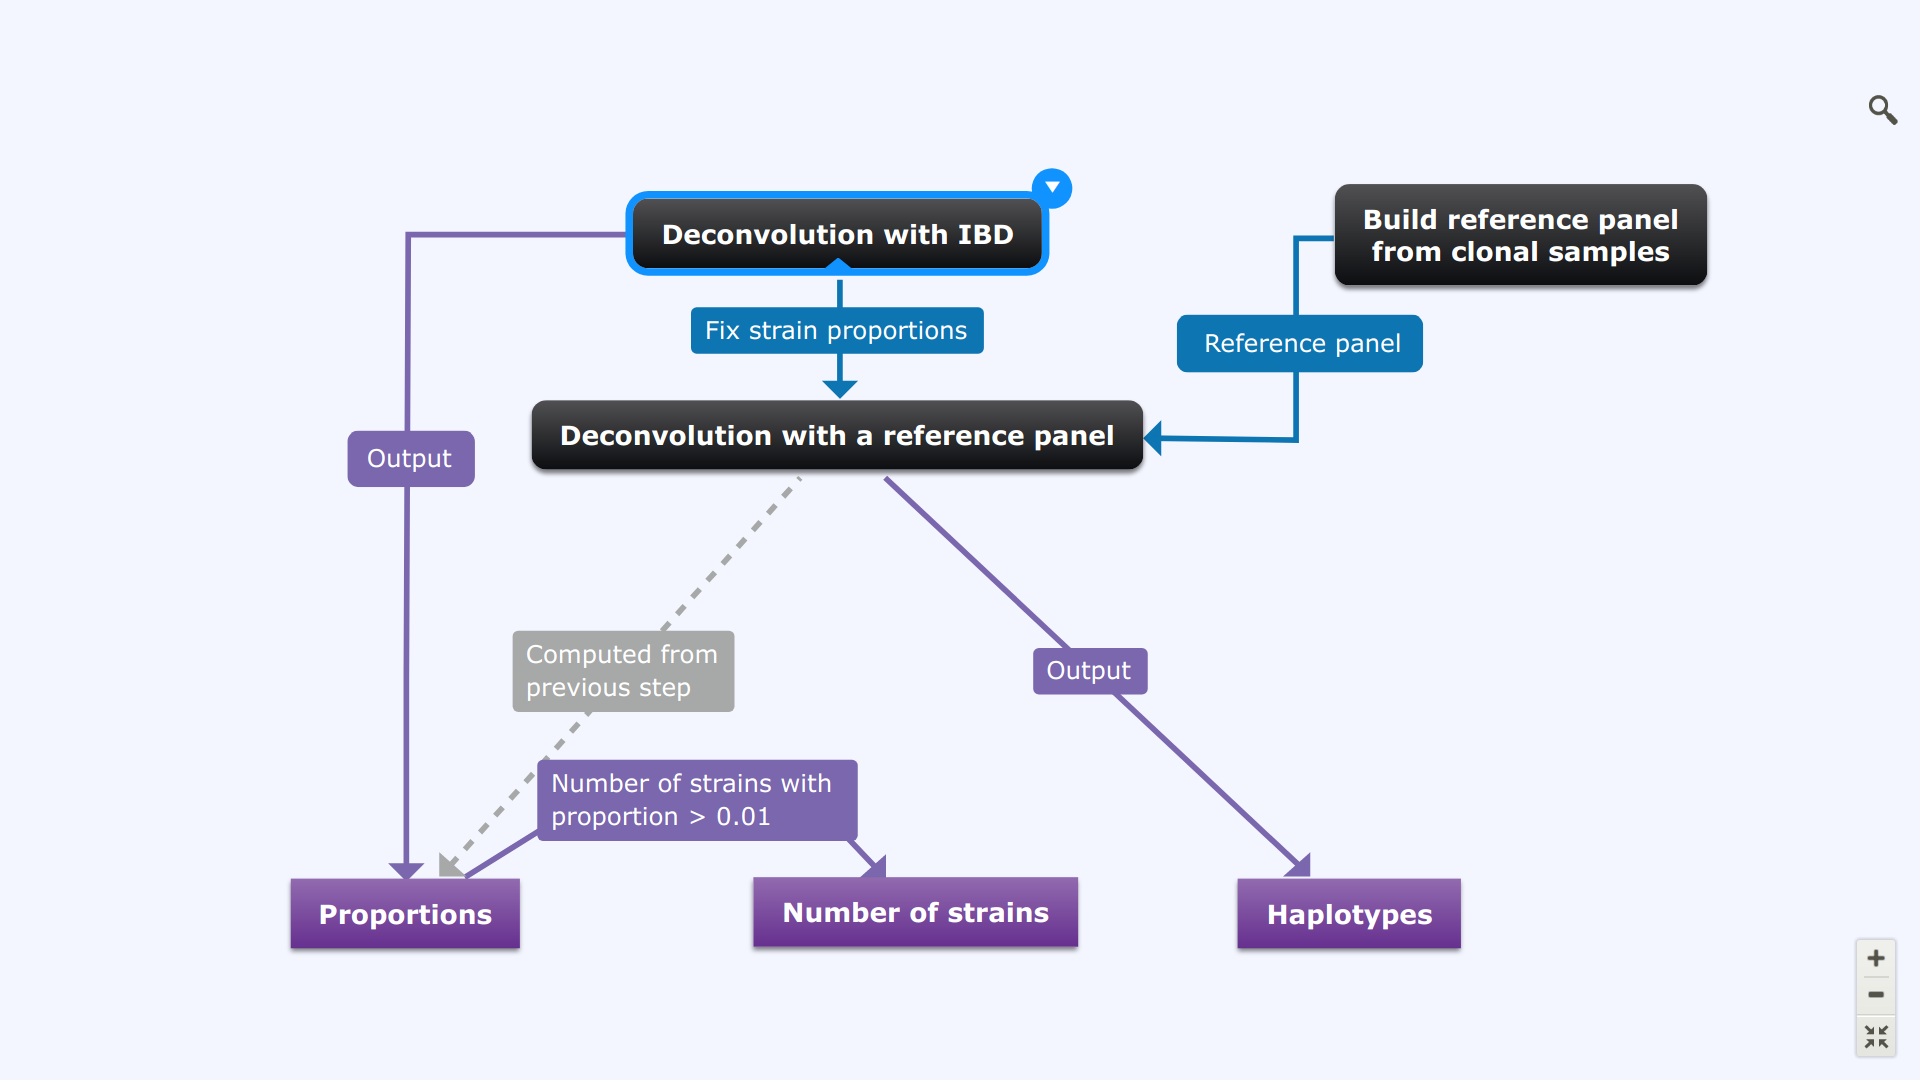
\includegraphics[width=0.7\textwidth]{scheme.png}}
  \\
  \subfloat[][]{\includegraphics[width=0.6\textwidth]{{myring.ring}.png}}
  \caption{IBD enchanced DEploid pipepline and results. (a) Schematic approach. Black boxes indicate the key deconvolution steps when our program DEploid is used. Boxes in blue and purple represent the input and output respectively at each step. (b) Highlights of the genome diversity within the mixed sample across the genome. This deconvolution example of field sample PD0577-C suggest that there are three related strains within this isolate, with proportions of 22/52/26\%. The outer ring show expected WSAF (blue) and observed WSAF (red) across the genome. This inner ring marks the IBD regions of the three strains: green colored segments mark the regions where all three strains are IBD; yellow, orange and dark orange segments identify the regions where pair of strains are IBD.}\label{fig:scheme}
\end{figure}

We benchmark our new method with DEploid implementation described by \citep{Zhu2017}

\narrative{2. Joint estimation of IBD, strains and proportions.  Details in SOM.  Figure 1b.  Example deconvolution in real data showing IBD transitions.}


\subsection{Method validation}

Similar to \citep{Zhu2017}, we validate our method using the same set of {\it in vitro} mixtures created by \citep{Wendler2015} to simulate mixed infections. DNA was extracted from four laboratory parasite lines: 3D7, Dd2, HB3 and 7G8, experimentally mixed in different proportions (see Fig. 1), and submitted to the MalariaGEN pipeline (MalariaGEN, 2008) for Illumina sequencing and genotyping (Manske et al., 2012).
{\it in vitro} sample test.

The lab strain mixture reflects an artificial situation that is unlikely in the field. To assess the performance of DEploid in realistic settings, we created in silico mixtures from 212 clonal samples of Asian origin with two proportions (25/75\% and 45/55\%) for 8071 sites from Chromosome 14. A further 20 randomly chosen samples were used for the reference panel. To simulate data, we used empirical read depths and drew read counts for the two alleles from the binomial proportions given by Equation (4). DEploid correctly recovered the number of strains and proportions. As expected, we observed more switches and genotype errors in 45/55\% mixtures than 25/75\% mixtures, with means of 24.3 and 0.57 for switch errors, and 0.013 and 0.0042 for per-site genotype errors (combining isolated and strain drop-out errors) respectively (Fig. 4). In summary, because field samples are likely to contain haplotypes much more closely related to each other than the artificial lab strain mixtures, we consequently expect high genotype accuracy and, at least for samples with unbalanced mixtures, very low switch error rates.



\narrative{3. Validation through empirical data analysis and simulation.  Figure 2 showing simulation results.  Supplementary Figure 1 showing effective k under DEploid with and without IBD.}
\begin{figure}[htp]
  \centering{}
  \subfloat[][]{
  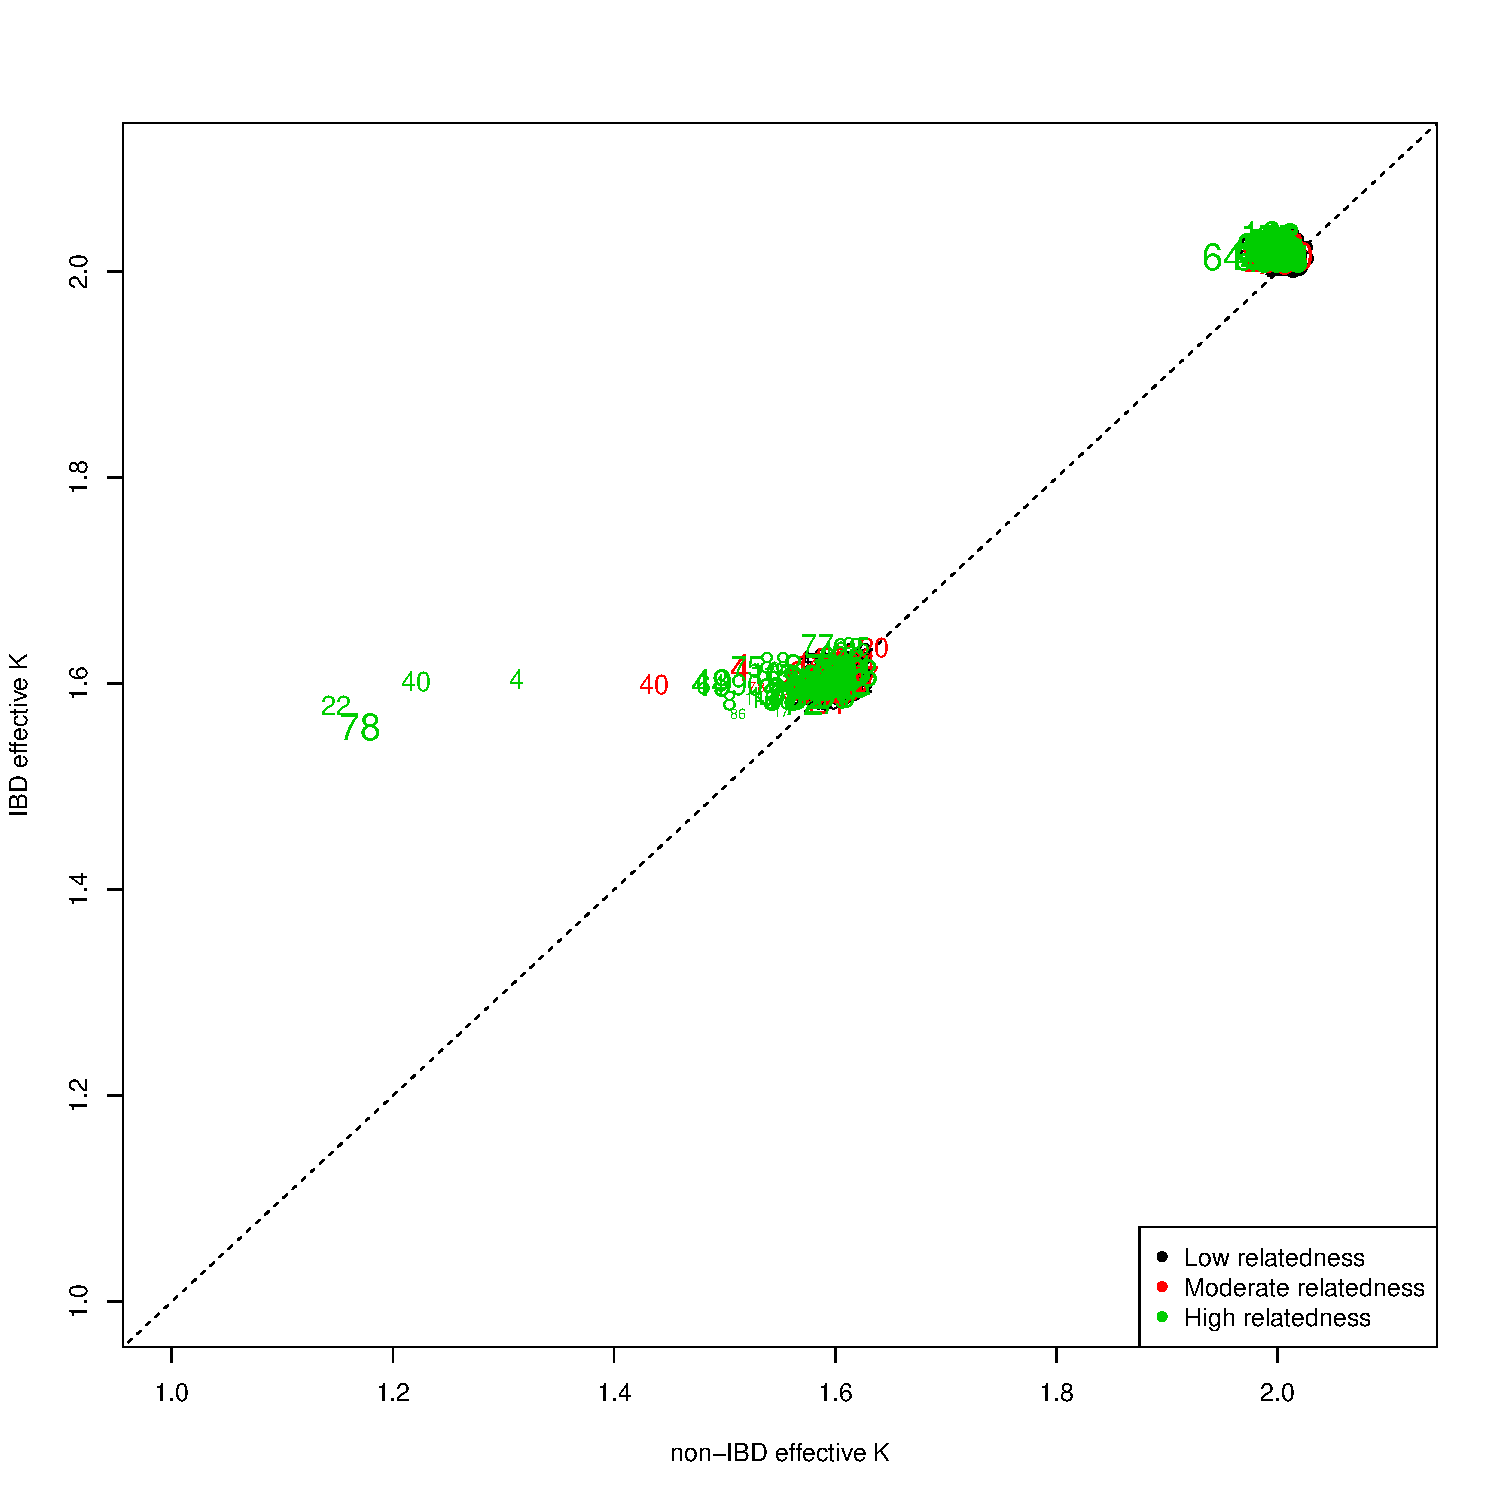
\includegraphics[width = 0.45\textwidth]{diagnositicPlot_of_effK_final.pdf}
  }
  \subfloat[][]{
  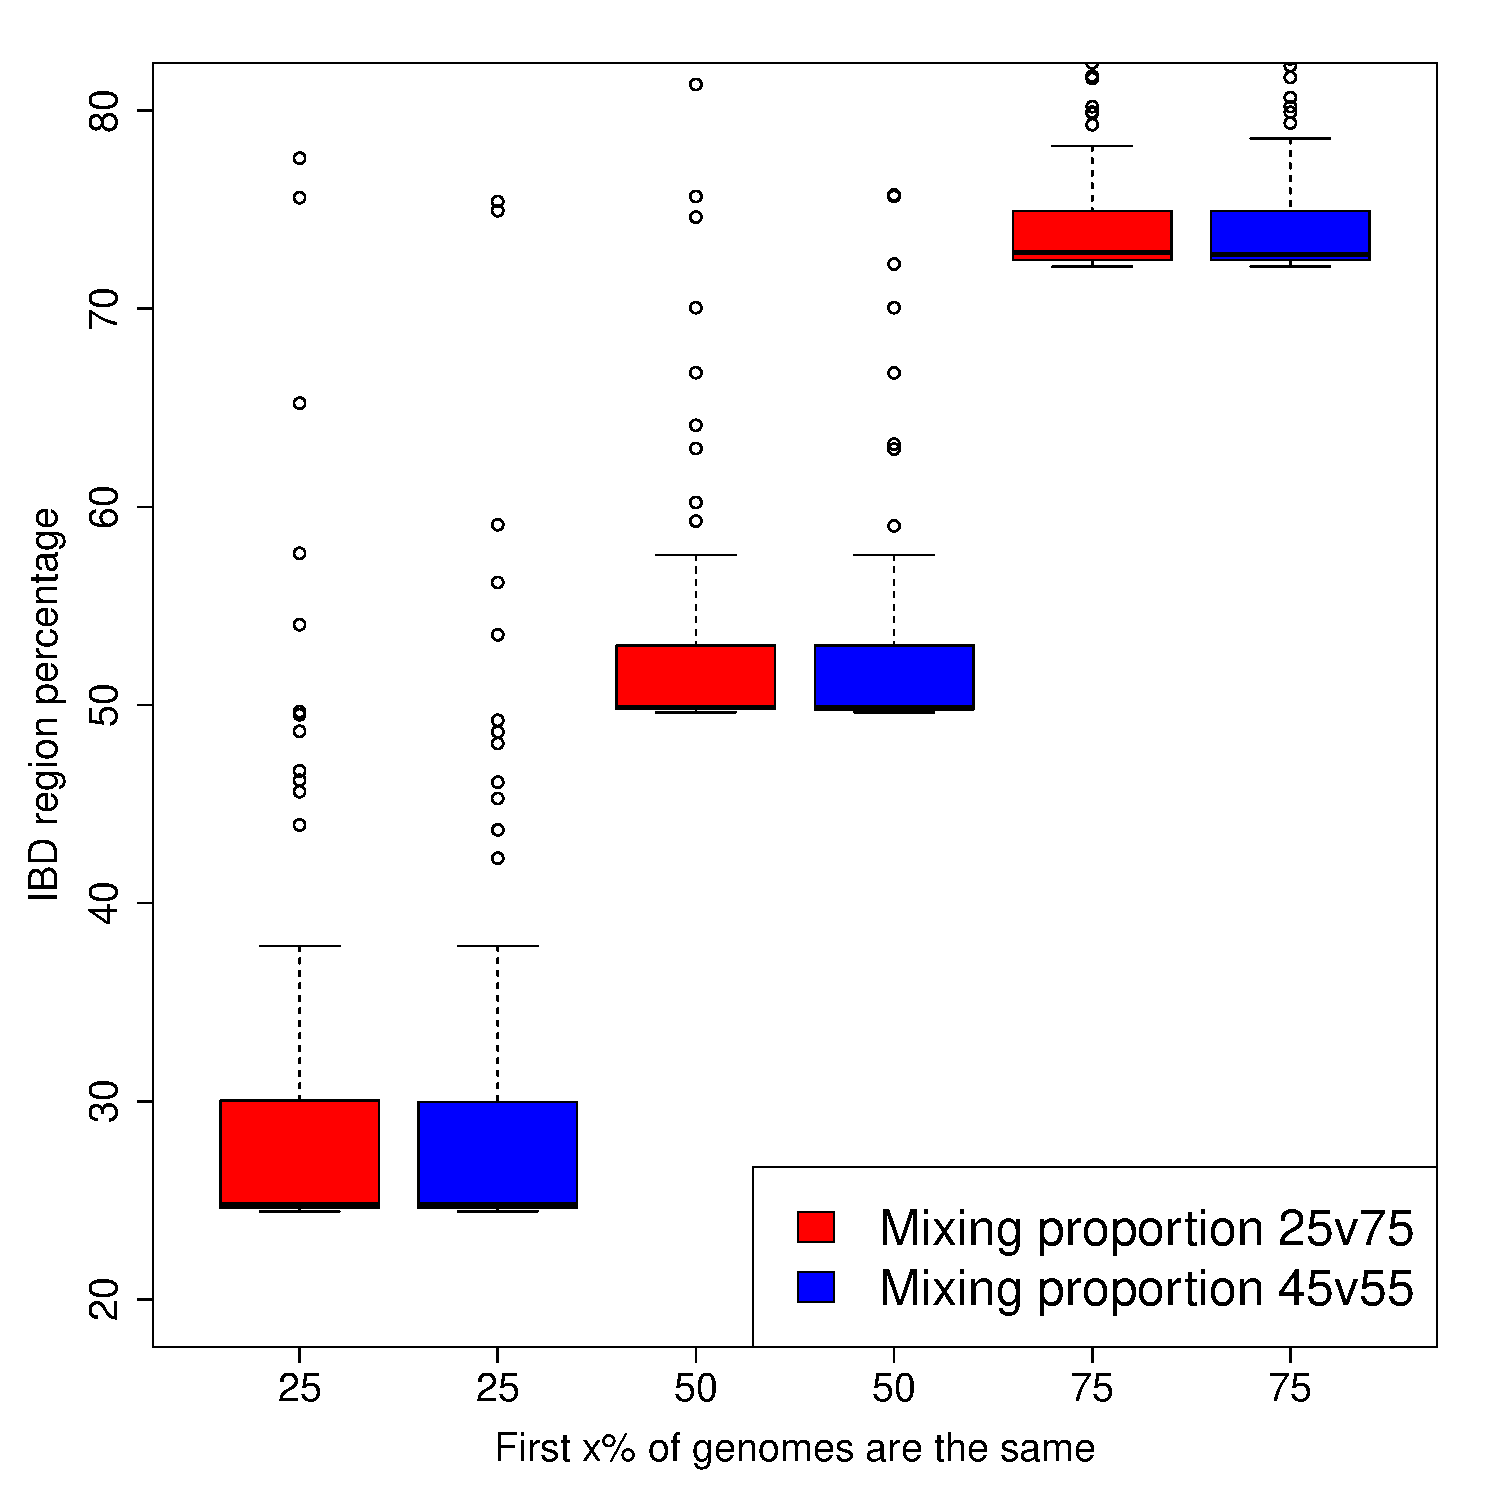
\includegraphics[width = 0.45\textwidth]{IBDprobs.pdf}
  }\\
  \subfloat[][]{
  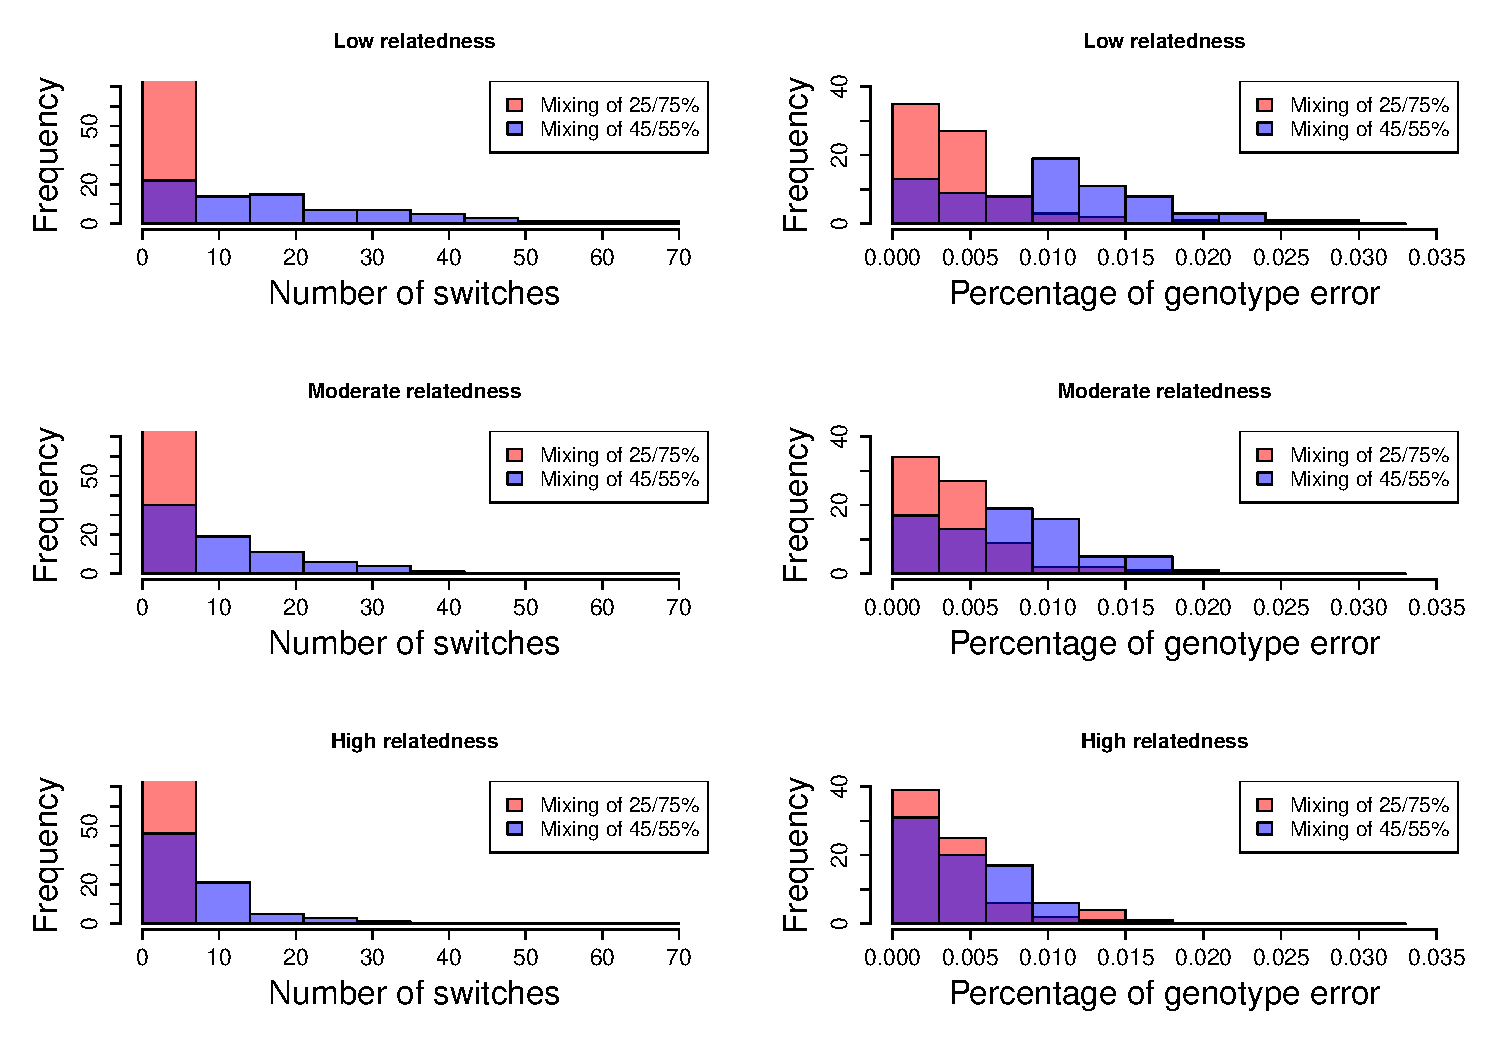
\includegraphics[width = 0.8\textwidth]{IBDHapError.pdf}
  }
  \caption{Simulation results}
\end{figure}


\section{Application to Pf and Pv data}
\narrative{1. Data source and preparation (i.e. cleaning).  Supplementary Figure 2 on importance of strong variant filtering.}

Background of two dataset, different filtering step was applied.


\narrative{2. Summary of findings within Pf and Pv. Figure 3: Rates of co-infection by geography and species.}

\begin{figure}[htp]
\centering
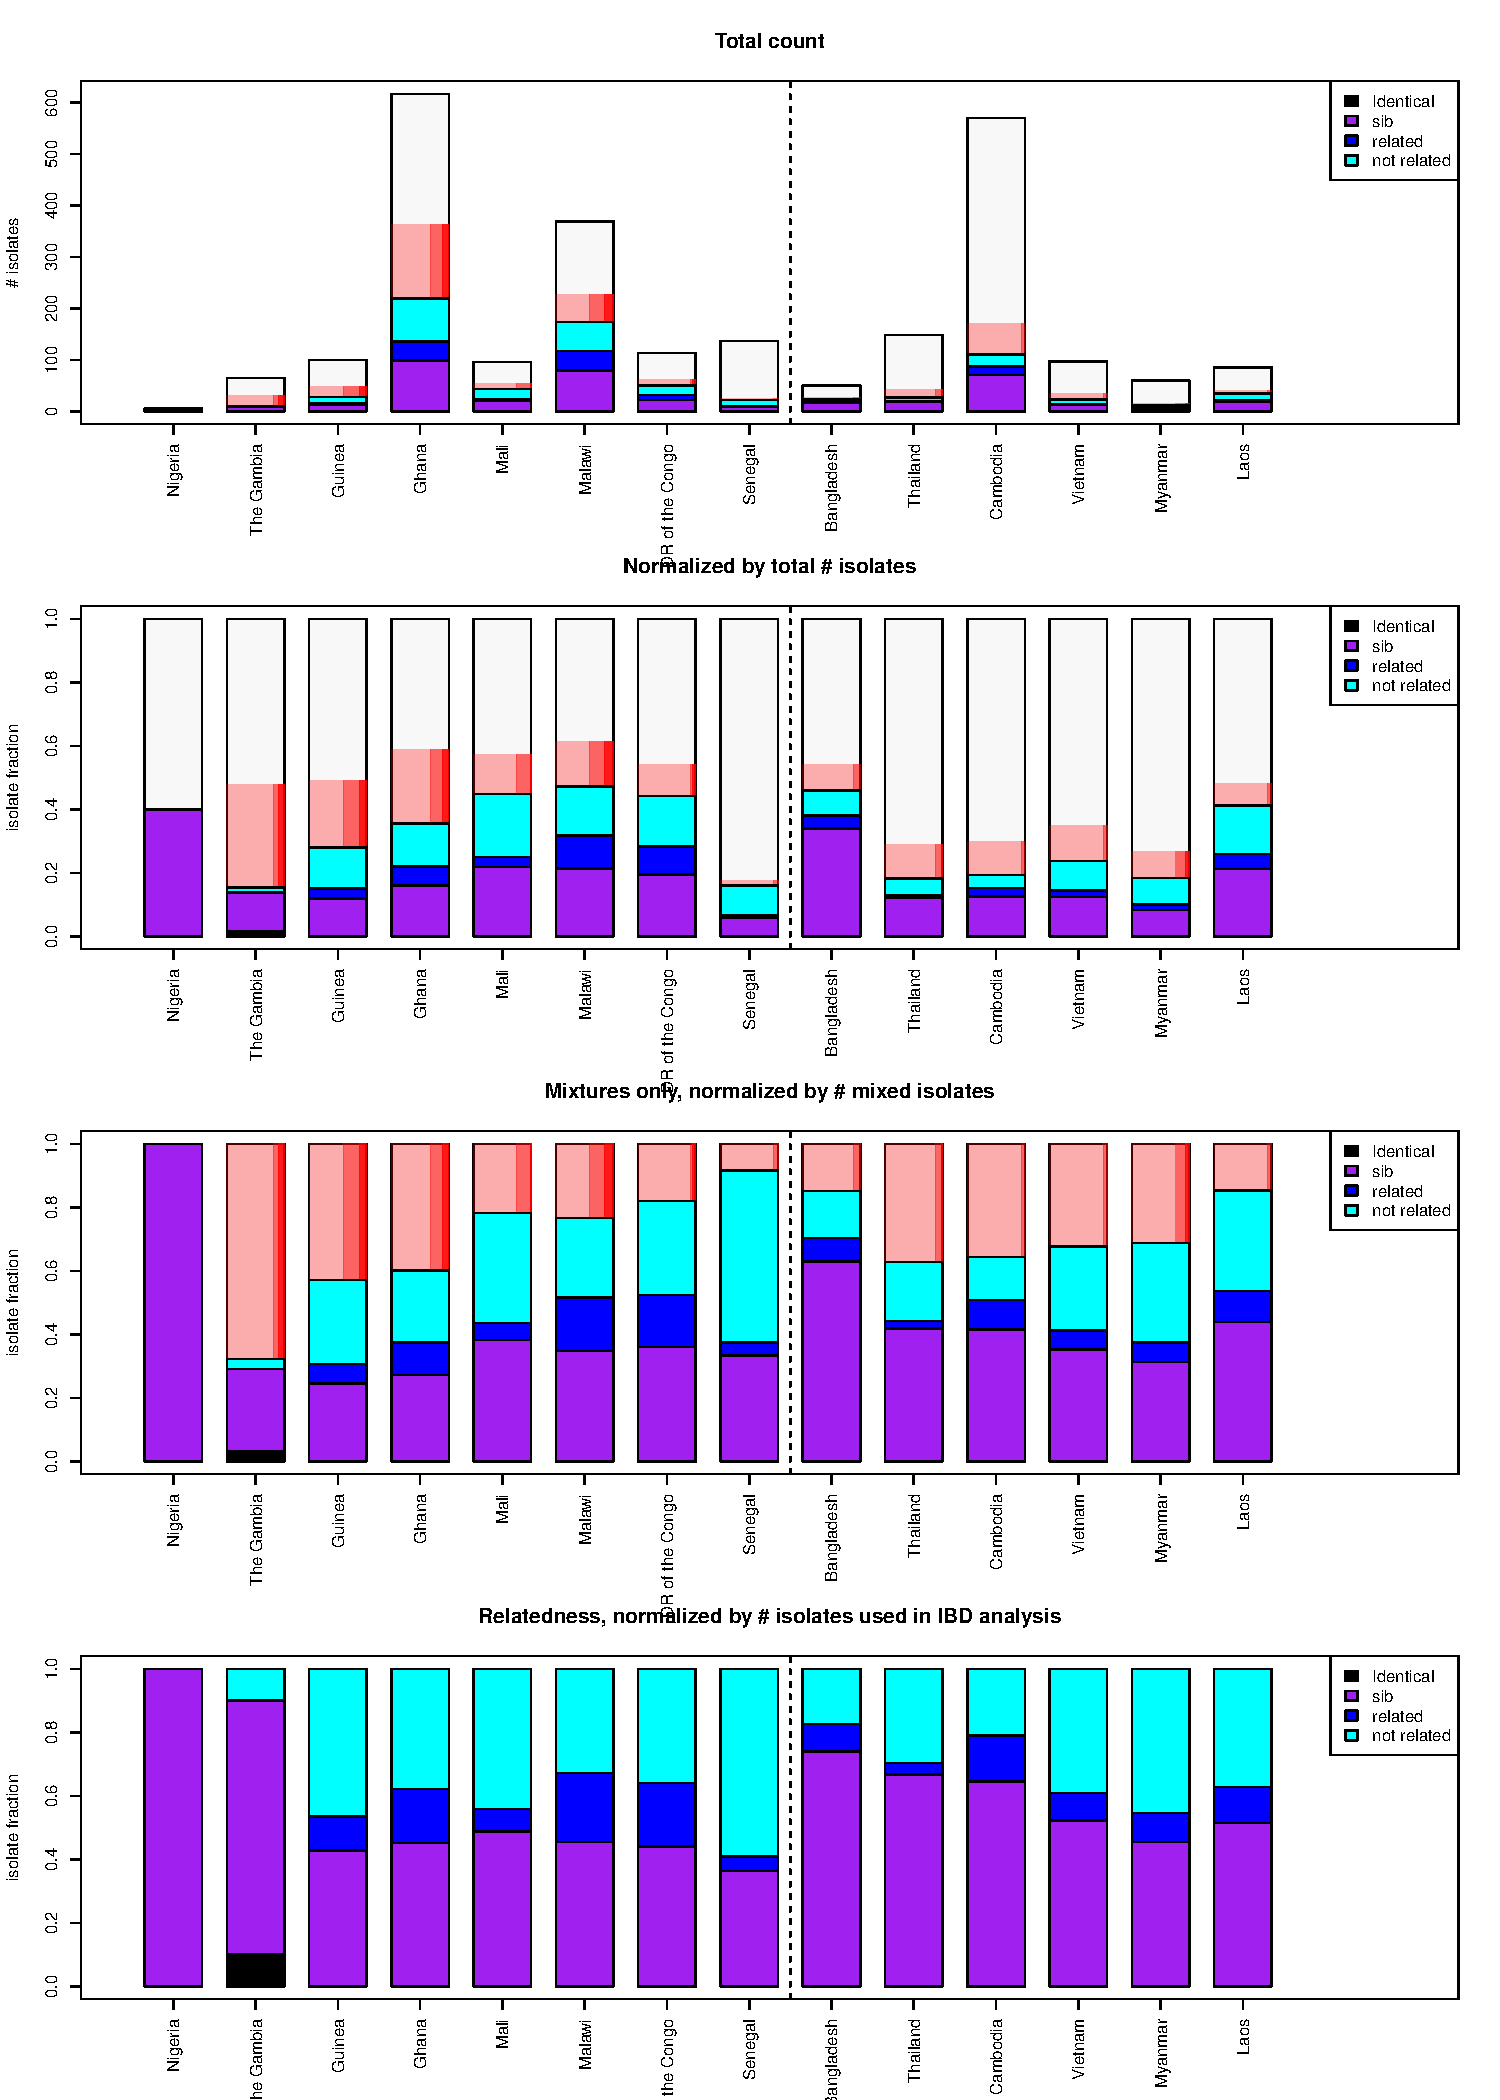
\includegraphics[width=0.8\textwidth]{pf_mixed_strutures_old.pdf}
\caption{}
\end{figure}



\narrative{3. Summary of findings about relatedness within mixed infections.  Figure 4.  Relatedness structure histogram showing peaks at 0.25, 0.5, etc. and relationship between mixed infection rate and sib-strain.}

\begin{figure}[htp]
  \centering{}
  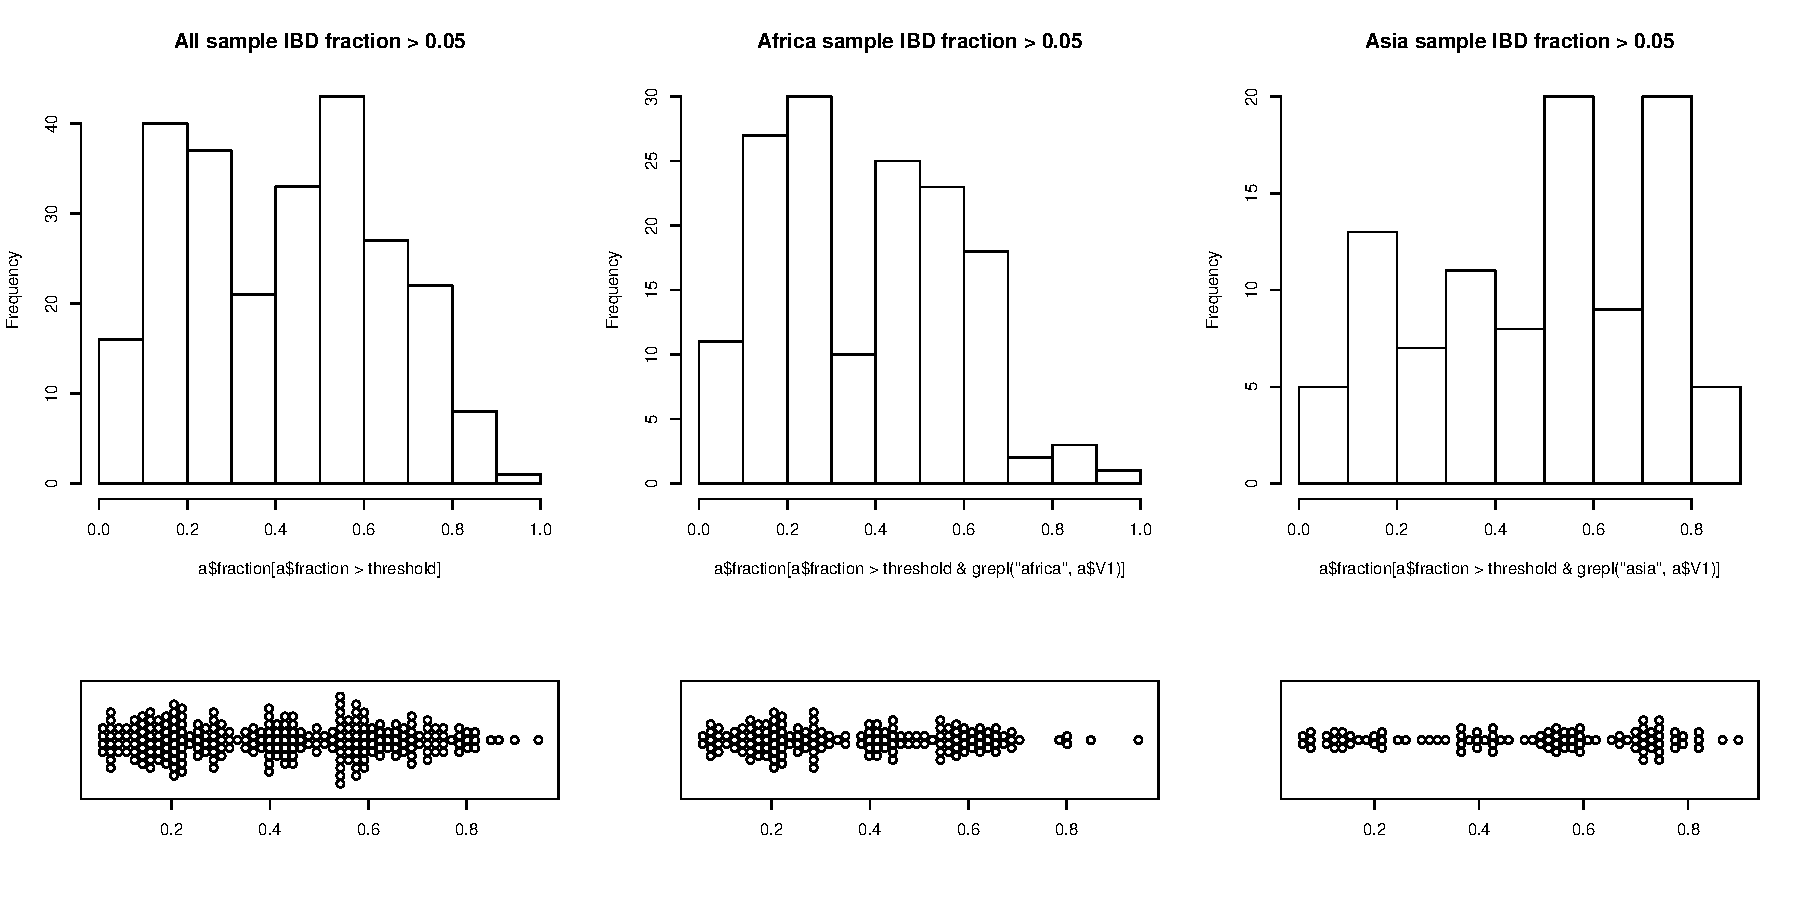
\includegraphics[width=0.8\textwidth]{IBD_fraction_hist.pdf}
  \caption{Schematic approach. Black box indicates when DEploid is used. Purple box indicates output.}\label{fig:IBD_frac_hist}
\end{figure}


\narrative{4. Simulation results to analyse the relationship between prevalence, mixed infection rate and sib-strain rate.  Figure 5 summarising simulations.}

\section{Discussion}


\narrative{1. Recap of main findings.}

\narrative{2. Relationship of mixed infection to prevalence v population size from simulations and interpretation of empirical data in the light of this.}

\narrative{3. Interpretation of within and between sample relatedness – does it reflect some feature of underlying biology?}

\narrative{4. Directions for integrating genomic data into efforts to map spatial and temporal changes in prevalence.}





\section{ACKNOWLEDGMENTS}
We thank the Pf3k consortium for valuable insights. The project is funded by the Wellcome Trust grant [100956/Z/13/Z] to GM.

\section{DISCLOSURE DECLARATION}
None declared.


\begin{thebibliography}{}

\bibitem[\protect\citeauthoryear{Browning and Browning}{Browning and
  Browning}{2007}]{Browning2007}
Browning, S. R. and B.~L. Browning (2007)
\newblock Rapid and accurate haplotype phasing and missing-data inference for
  whole-genome association studies by use of localised haplotype clustering.
\newblock {\em Am. J. Hum. Genet.\/}~{\em 81\/}(5), 1084--1097.

\bibitem[\protect\citeauthoryear{Chang}{Chang et~al.}{2017}]{Chang2017}
\textcolor{black}{Change, H.~H. et al. (2017)
\newblock THE REAL McCOIL: A method for the concurrent estimation of the complexity of infection and SNP allele frequency for malaria parasites.
\newblock {\em PLoS Comput. Biol.\/}~{\em 13\/}(1), e1005348.}

\bibitem[\protect\citeauthoryear{Collins}{Collins}{2012}]{Collins2012}
Collins, W. E. (2012).
\newblock {\it Plasmodium knowlesi}: A malaria parasite of monkeys and humans.
\newblock {\em Annual Review of Entomology}~{\em 57\/}, 107--21.

\bibitem[\protect\citeauthoryear{Galinsky et~al.}{Galinsky et~al.}{2015}]{Galinsky2015}
Galinsky, K. {\em et al}. (2015)
\newblock COIL: a methodology for evaluating malarial complexity of infection using likelihood from single nucleotide polymorphism data.
\newblock {\em Malar. J.\/}~{\em14\/}(4), 1--9.

\bibitem[\protect\citeauthoryear{Hinch}{Hinch}{2011}]{Hinch2011}
Hinch, A. G. {\em et al}. (2011))
\newblock The landscape of recombination in African Americans.
\newblock {\em Nature\/}~{\em 476}, 170--175.

\bibitem[\protect\citeauthoryear{Henden}{Henden}{2016}]{Henden2016}
Henden, L. {\em et al}. (2016))
\newblock Detecting selection signals in {\it Plasmodium falciparum} using identity-by-descent analysis,
\newblock {\em bioRxiv.\/}, 088039.

\bibitem[\protect\citeauthoryear{Jiang}{Jiang}{2011}]{Jiang2011}
Jiang, H. {\em et al}. (2011)
\newblock High recombination rates and hotspots in a {\it Plasmodium falciparum} genetic cross.
\newblock {\em Genome Biology.\/}~{\em 12}, R33.

\bibitem[\protect\citeauthoryear{Lopez}{Lopez}{2012}]{Lopez2012}
Lopez A. {\em et al}. (2012)
\newblock Genetic diversity of {\it Plasmodium vivax} and {\it Plasmodium falciparum} in Honduras.
\newblock {\em Malaria Journal.\/}~{\em 11}, 391.

\bibitem[\protect\citeauthoryear{Manske et~al.}{Manske et~al.}{2012}]{Manske2012}
Manske, M. {\em et al}. (2012)
\newblock Analysis of plasmodium falciparum diversity in natural infections by
  deep sequencing.
\newblock {\em Nature\/}~{\em 487\/}(7407), 375--379.

\bibitem[\protect\citeauthoryear{Miles et~al.}{Miles et~al.}{2016}]{Miles2016}
Miles, A. {\em et al}. (2015)
\newblock Indels, structural variation, and recombination drive genomic diversity in {\it Plasmodium falciparum}.
\newblock {\em Genome Res.\/}~{\em26\/}, 1288--1299.

\bibitem[\protect\citeauthoryear{Mu}{Mu}{2005}]{Mu2005}
Mu, J. {\em et al}. (2005)
\newblock Recombination Hotspots and Population Structure in {\it Plasmodium falciparum}.
\newblock {\em PLOS Biology.\/}~{\em 3}, e335.

\bibitem[\protect\citeauthoryear{Mueller et~al.}{Mueller et~al.}{2007}]{Mueller2007}
Mueller, I. {\em et al}. (2007)
\newblock {\it Plasmodium malariae} and {\it Plasmodium ovale} -- the ``bashful'' malaria parasites.
\newblock {\em Trends in Parasitology}~{\em 23\/} (6), 278--283.

\bibitem[\protect\citeauthoryear{Nair et~al.}{Nair et~al.}{2014}]{Nair2014}
Nair, S. {\em et al}. (2014)
\newblock Single-cell genomics for dissection of complex malaria infections
\newblock {\em Genome research.\/}~{\em 24}, 1028--1038.

\bibitem[\protect\citeauthoryear{Neafsey}{Neafsey}{2012}]{Neafsey2012}
Neafsey, D. {\em et al}.(2012)
\newblock The malaria parasite {\it Plasmodium vivax} exhibits greater genetic diversity than {\it Plasmodium falciparum}.
\newblock {\em Nature Genetics\/}~{\em 44\/}(9), 1046--1052.

\bibitem[\protect\citeauthoryear{O'Brien et~al.}{O'Brien et~al.}{2016}]{Jack2016}
O'Brien D. J. {\em et al}. (2016)
\newblock Inferring Strain Mixture within Clinical {\em Plasmodium falciparum} Isolates from Genomic Sequence Data.
\newblock {\em PLoS Comput. Biol.\/}~{\em 12\/}(6): e1004824.

\bibitem[\protect\citeauthoryear{O'Brien et~al.}{O'Brien et~al.}{2015}]{Jack2016Inbreeding}
O'Brien D. J. {\em et al}. (2016)
\newblock Approaches to estimating inbreeding coefficients in clinical isolates of {\it Plasmodium falciparum} from genomic sequence data.
\newblock {\em Malaria Journal\/}~{\em 15}:473.


\bibitem[\protect\citeauthoryear{Pearson et~al.}{Pearson et~al.}{2016}]{Pearson2016}
Pearson, R. D. {\em et al}. (2016)
\newblock {Genomic analysis of local variation and recent evolution in {\it Plasmodium vivax}}.
\newblock {\em Nat. Genet.\/}~{\em 48}, 959--964.


\bibitem[\protect\citeauthoryear{Rutledge}{Rutledge et~al.}{2017}]{Rutledge2017}
Rutledge. G. G., {\em et al}. (2017)
\newblock {\it Plasmodium} malariae and P. ovale genomes provide insights into malaria parasite evolution
\newblock {\em Nature.\/}~{\em 542}, 101--104.


\bibitem[\protect\citeauthoryear{Pf3k}{Pf3k}{2016}]{Pf3k2016}
The Pf3k Project: pilot data release 5 (2016)
\newblock {www.malariagen.net/data/pf3k-5} [accessed 1 June 2016]


\bibitem[\protect\citeauthoryear{Schaffner}{Schaffner}{2017}]{Schaffner2017}
Schaffner, S. F. {\em et al.} (2017)
\newblock {hmmIBD: software to infer pairwise identity by descent between haploid genotypes},
\newblock {\em bioRxiv}, doi:10.1101/188078.

\bibitem[\protect\citeauthoryear{Wegmann}{Wegmann}{2011}]{Wegmann2011}
Wegmann, D. {\em et al}.(2011)
\newblock Recombination rates in admixed individuals identified by ancestry-based inference.
\newblock {\em Nature Genetics\/}~{\em 43\/}, 847--894.

\bibitem[\protect\citeauthoryear{Wendler}{Wendler}{2015}]{Wendler2015}
Wendler, J. (2015)
\newblock {\em Accessing complex genomic variation in} {P}lasmodium falciparum {\em natural infection}.
\newblock {Ph.\ D. thesis, University of Oxford.}

\bibitem[\protect\citeauthoryear{WHO}{WHO}{2016}]{WHO2016}
WHO. (2016)
\newblock {World Malaria Report 2015}.
\newblock {\em World Health Organization\/}.

\bibitem[\protect\citeauthoryear{Wong}{Wong}{2017}]{Wong2017}
Wong W., {\em et al}. (2017)
\newblock Genetic relatedness analysis reveals the cotransmission of genetically related {\it Plasmodium falciparum} parasites in Thiès, Senegal.
\newblock {\em Genome Medicine.\/}~{\em 9}:5. doi:10.1186/s13073-017-0398-0.

\bibitem[\protect\citeauthoryear{Zhu, Garcia, McVean}{Zhu et~al.}{2017}]{Zhu2017}
Zhu, J. S., {\em et al} (2017)
\newblock {Deconvoluting multiple infections in {\it Plasmodium falciparum} from high throughput sequencing data}.
\newblock {\em Bioinformatics\/}~{\em \/}btx530. doi: https://doi.org/10.1093/bioinformatics/btx530

\end{thebibliography}

\end{document}
